\chapter{From recorded counts to a classical explanation bound}
\label{rr:explanation}

An observed failure of a model should say more than ``the model is wrong.''
The sharp reset bound provides a quantitative alternative: a classical
explanation must permit a certain reset mismatch or a sufficiently large
peak rate of crossing the observed boundary. This chapter connects that
statement to finite data. It does not infer entropy production, total jump
activity or quantumness from a binary record.

\section{The contract for inference}
The reference preparation is supported inside an observed region $B$ and
the comparison preparation outside $B$. Both use the same independent
uniform readout clock on $[0,T]$. A fresh fair coin selects the arm on each
trial. Encode success as $Y$ in the comparison arm and $1-Y$ in the reference
arm. With observed contrast
$C_{\rm obs}=p_B^{\rm reference}-p_B^{\rm comparison}$, the encoded success
probability is $\theta=(1-C_{\rm obs})/2$.

The common detector gain $g\in(0,1]$ is calibrated. Let $\delta\geq0$ bound
the remaining discrepancy of the observed contrast from $gH/T$, including
any propagated preparation, clock and setting-dependent detector errors.
Thus $C_{\rm obs}\geq gH/T-\delta$. A shared fixed detector offset cancels.
For reset inference assume uniform entrance and exit caps $a,b$ and the
Markov or regenerative entrance assumptions of the sharp reset theorem.
These caps concern every relevant hidden state or history; observed average
rates do not establish them.

The outside-$B$ condition matters. A coherent quadrature comparison
preparation generally has nonzero initial occupancy of $B$ and needs the
partially occupied preparation version of the bound. It cannot be inserted
into the outside-$B$ formula solely because it gives a larger signal.

\section{A fixed-horizon confidence statement}
Fix $n$ before data collection and let $S$ be the encoded success count.
Compute a rational lower confidence endpoint $q(S)$ by inverting the upper
binomial tail. The implementation returns a conservative dyadic endpoint
with
\[
 \Pr_{\operatorname{Bin}(n,q(S))}(S'\geq S)\leq\alpha
\]
whenever the endpoint is positive. For a stable Bernoulli mean, standard
one-sided test inversion gives $\Pr\{q(S)>\theta\}\leq\alpha$.
More generally, a candidate uniform conditional upper bound
$\Pr(R_k=1\mid\mathcal F_{k-1})\leq\theta_0$ is stochastically dominated
by $\operatorname{Bin}(n,\theta_0)$. The same procedure therefore excludes
such upper bounds with type-I error at most $\alpha$, without claiming that
an arbitrary time-varying process has a single unknown mean.

On the corresponding confidence event,
\[
 C_{\rm obs}\leq1-2q(S),\qquad
 H\leq H_+:=\frac{T[1-2q(S)+\delta]}{g}.
\]
Let $G$ and $K$ have the meanings established in the sharp reset theorem,
so that $H\geq G-\eta K$. If $K>0$, every compatible explanation must obey
\begin{equation}\label{rr:eta-inference}
 \eta\geq\max\left\{0,\frac{G-H_+}{K}\right\}.
\end{equation}
The software uses a rational lower enclosure $G_-$ and an upper enclosure
$K_+$, giving the conservative numerator $(G_--H_+)_+$ divided by $K_+$.
If the resulting lower bound exceeds one, the declared bounded-hazard
classical class is incompatible at the stated error level. A zero result
is inconclusive. When $K=0$, a strictly positive numerator already contradicts
the contract.

This remains an exclusion of nested physical model classes when conditional
probabilities vary between trials: a proposed common defect cap $\eta_0$
implies a uniform bound on each encoded success probability, to which the
binomial domination argument applies. Calibration envelopes must hold in the
conditional form needed for that argument. A separately justified joint
calibration failure probability is added once.

\section{A required peak intensity without assuming a reset law}
Dropping the reset condition gives the sharp inequality
\[
 \frac HT\geq\frac{A_a(T)+A_b(T)}T-1,
 \qquad A_c(T)=\int_0^T e^{-cs}\,ds.
\]
If both macro-crossing intensities are at most $\lambda$, then
\[
 \frac HT\geq f(\lambda T),\qquad
 f(z)=\frac{2(1-e^{-z})}{z}-1,
 \qquad f(0)=1.
\]
The function decreases strictly from one to minus one. Indeed its derivative
has the sign of $(z+1)e^{-z}-1<0$ for $z>0$. Hence a calibrated upper
contrast $C_+=H_+/T\in(-1,1)$ forces
\[
 \lambda\geq f^{-1}(C_+)/T.
\]
The implementation brackets this root using rational exponential bounds.
This is a necessary peak macro-crossing intensity for a classical explanation.
It is not a bound on average total dynamical activity, power or dissipation.
This unrestricted-reset inequality also holds for time-dependent and
history-dependent classical processes with the specified conditional
crossing-hazard bounds. Memory alone does not evade a valid hazard cap.

\section{A fully reproducible count example}
Take the explicitly synthetic count $S=343$ out of $n=600$ records, with
$T=9/4$, $g=9/10$, $\delta=1/1000$ and $\alpha=1/20$. The count was chosen
as an illustrative rounded model mean; it is not a physical measurement.
The exported exact certificates imply the following conservative consequences:
\begin{center}
\begin{tabular}{ll}
\toprule
Supplied classical contract & Consequence of these synthetic counts\\
\midrule
$a=b=1/2$ & No compatible reset defect in $[0,1]$\\
$a=b=1$ & Reset defect at least $0.604$\\
$a=b=2$ & Reset defect at least $0.162$\\
No supplied cap; unrestricted reset & Required peak intensity above $0.812$\\
\bottomrule
\end{tabular}
\end{center}
Rates use the reciprocal of the declared time unit. Rounded numbers here are
weaker than the rational certified bounds. They demonstrate how a single
record can constrain competing explanations, rather than assigning an
unconditional physical interpretation to a rejected ideal model.

\begin{verbatim}
from fractions import Fraction as F
from constructive_access.robust import explanation

result = explanation.from_counts(
    records=600, successes=343,
    entrance_cap=1, exit_cap=1, time=F(9,4),
    gain=F(9,10), radius=F(1,1000), alpha=F(1,20))
\end{verbatim}
The record count must be fixed in advance for this routine. The sequential
statistics module supplies separate time-uniform procedures; repeatedly
inspecting the fixed-horizon endpoint and stopping opportunistically is not
covered. Physical assumptions and the provenance of actual counts remain
the user's responsibility at the apparatus boundary.

\begin{figure}[p]
\centering
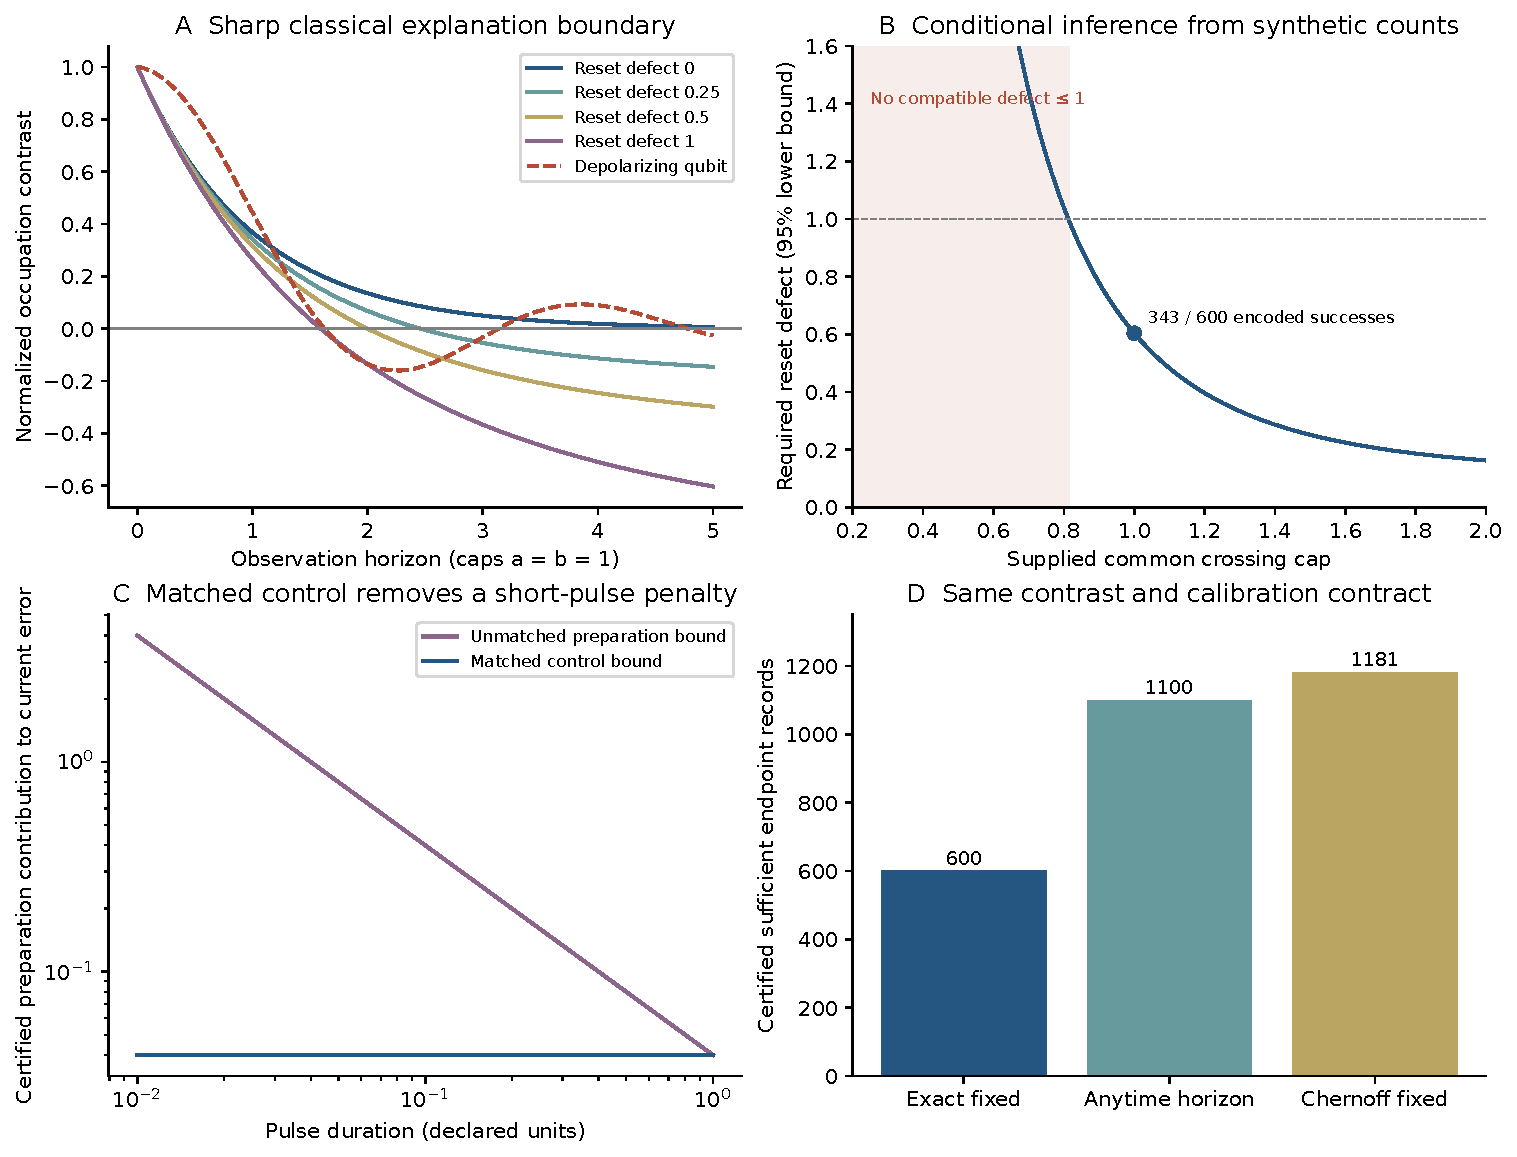
\includegraphics[width=\textwidth]{robust_results.pdf}
\caption{A: the sharp classical lower envelopes for several reset-defect caps,
with a depolarizing-qubit contrast as a model illustration. B: the required
reset defect from explicitly synthetic counts, conditional on the supplied
common crossing cap; values above one exclude that cap. C: preparation-error
contributions alone, for discrepancy $0.01$, channel rates $3,1$ and retention
$1/2$; matching the native control removes the $1/t$ penalty in this bound.
D: sufficient fixed and anytime record budgets for the same declared contrast,
calibration and 5\% error targets. The anytime bar is a guaranteed horizon,
not an expected stopping time. No panel contains physical measurements.}
\label{rr:overview}
\end{figure}

\section{A laboratory route that does not assume hidden reset purity}
The realization-size test asks a different question from reset-defect inversion.
Its target is whether a single homogeneous classical Markov description with
at most three states can explain the records. It needs two repeatable
preparation commands, one fixed binary readout, a common evolution setting,
and an independent clock. The preparations may be mixed and the readout may be
noisy. Hidden environmental and controller states that affect the dynamics
belong to the realization being bounded.

There are four equally randomized arms: each preparation is measured either
at the common reference time or after an independent uniform hold in $[0,T]$.
Use fresh trials and perform only the terminal measurement. The immediate and
delayed observations come from different trials; a baseline measurement must
not be inserted into the delayed evolution. Common latency is allowed when it
is shared by all arms and independent of the hold-time draw. Calibration must
bound changes between the arms, including preparation drift, detector drift,
and arm-dependent dynamics. A fixed detector's intrinsic noise is already
covered by the theorem.

The statistical chapter gives a complete four-arm encoding and a predeclared
record-count certificate. Its exact qubit alternative is a feasibility
prediction. The laboratory decision is a rejection of the calibrated
three-state description, not confirmation of a unique quantum mechanism.
A classical four-state control and a time-dependent three-state control test
how the interpretation fails when the relevant model assumptions change.
Time stamps should be retained for diagnostics, even when the stated decision
uses only the integrated statistic; no time-bin postselection belongs in that
decision rule.

\begin{figure}[htbp]
\centering
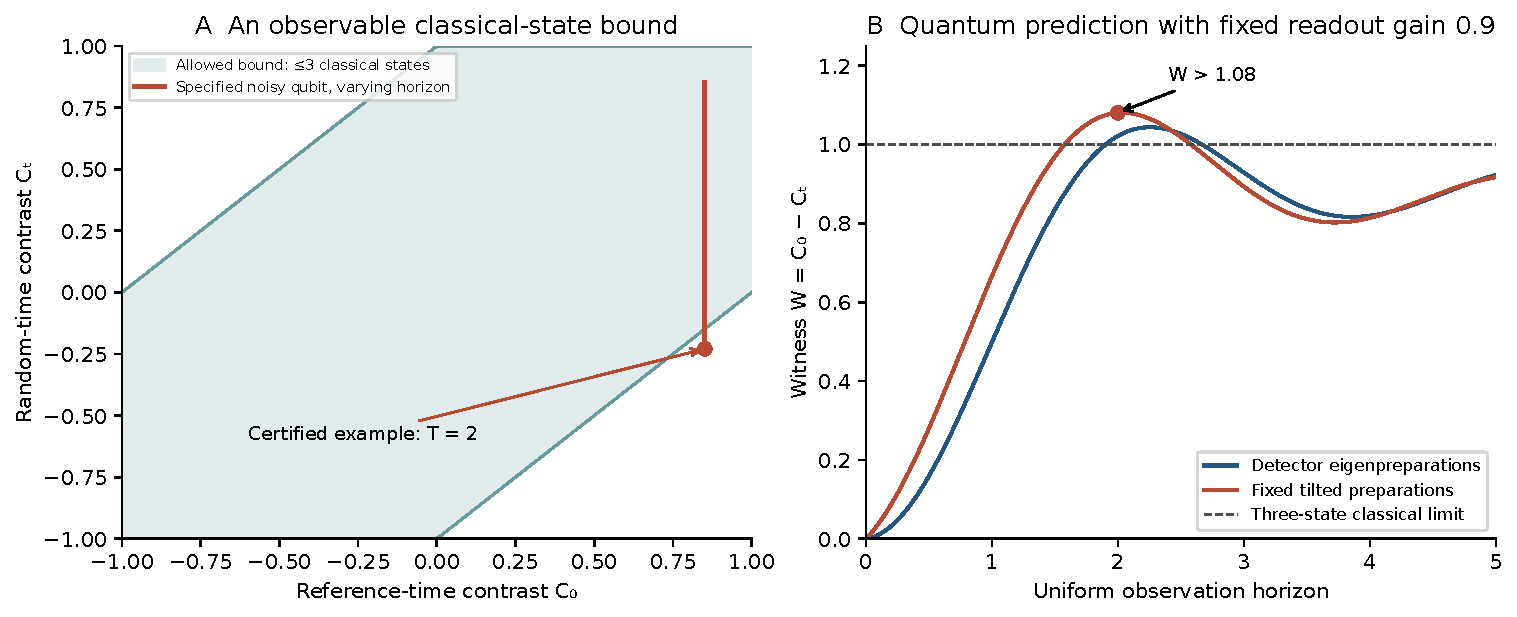
\includegraphics[width=\textwidth]{dimension_witness.pdf}
\caption{The integrated realization-size witness. The shaded strip contains
all common homogeneous classical models with at most three states, arbitrary
preparations and a fixed stochastic binary detector. The displayed qubit model
leaves this strip. The two quantum curves use different fixed preparation
pairs; neither is an experimental dataset or a claim of global optimality.}
\label{rr:dimension-figure}
\end{figure}

\section{From required records to a physical energy budget}
Record count, elapsed evolution, and energy answer different questions. Suppose
an independently calibrated apparatus contract supplies a gross preparation
and readout energy cap $E_0$ per trial and a gross holding-power cap $P_{\max}$.
Include any clock or controller expenditure covered by these caps, and write
$E_{\rm cal}$ for separate calibration and setup expenditure. A fixed $N$-record
uniform-hold protocol then satisfies the deterministic bound
\[
 E_{\rm total}\leq E_{\rm cal}+NE_0+NP_{\max}T.
\]
For the four-arm realization-size protocol, half the trials have no additional
hold and half have mean hold $T/2$. Therefore
\[
 \mathbb E E_{\rm total}
 \leq E_{\rm cal}+NE_0+NP_{\max}T/4.
\]
The expectation is not a pathwise guarantee. Common latency and other overhead
must be added if they are absent from $E_0$.

The 600-record protected-preparation example has expected additional evolution
675 in its declared time unit. The 6000-record four-arm example at $T=2$ has
expected additional evolution 3000. The latter purchases freedom from exact
hidden preparation assumptions at a measurable acquisition cost. Neither
number is a joule value until the apparatus caps and time unit are calibrated.
No thermodynamic minimum or energy advantage over other dimension witnesses
is implied by these conditional accounting formulas.
